\chapter{Evaluierung}

\anno{ca. 10 Seiten} %Ref. hat 5


\section{Aufbau der Testumgebung}
% Aufbau der Messumgebung (1-2 Seiten)
%% Server/Betriebssystem
%% Datensätze
%% Anfragen
%% Systeme/Ansätze gegen die Sie sich vergleichen
%% Wie messen Sie? Methodik und Maßeinheiten?
%% Ist die Messung signifikant?
%% Hypothesen? Was erwarten Sie?

Sämtliche Tests in dieser Arbeit werden nach dem Muster aus Abbildung \ref{fig.pattern} aufgebaut. Ein \glqq Angreifer\grqq versucht einen Angriff auf das \glqq Opfer\grqq. Zum Vergleich folgt auf einen Test ohne \glqq Verteidiger\grqq immer ein gleicher Test mit Verteidiger.

\begin{figure}[bht]
  \begin{center}
    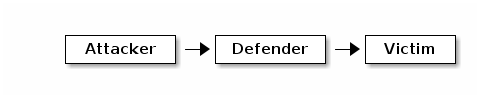
\includegraphics[width=10cm]{pattern}
    \caption{Muster für Tests}
    \label{fig.pattern}
  \end{center}
\end{figure}

\subsection{Attacker}
Angreifer können (handgeschriebene) Tests oder automatisierte Tools sein. Konkret werden in dieser Arbeit folgende Ausprägungen angewandt.

\subsubsection{Der manuelle Angriff}

Ein manueller Angriff ist ein exakt definierter Angriff der manuell ausgeführt wird. Der Ablauf ist dabei exakt in einer (Test-)Spezifikation beschrieben. Häufig existieren diese Tests in Form von Checklisten die vom einem Tester (Mensch) ab zuhaken sind. Mit Werkzeugen wie Selenium existieren auch Möglichkeiten diese Art von Test zu automatisieren. Der hier verwendete Test ruft im Grunde nur ein Formular auf und trägt in ein Textfeld einen mit einer SQl-Injektion versehenen bzw. manipulierten Wert ein. Im Anschluß wird das Formular abgesendet und der Rückgabewert kontrolliert.

\begin{neu}
manuellen Angriff beispielhaft erläutern; ggf. nochmal hinweis auf GrapheneTest (automatisierte Angriff); Hinweis/Übergang zu verschiedenen Beispiel-Datasets bzw. ref aus WAf-a-mole bzgl. verfügbarkeit
\end{neu}


\subsubsection{Der passive Angriff}
Im passiven Angriff wird der bereits aus Abschnitt \ref{ref:zap} bekannte \emph{Zed Attack Proxy} zwischen den Browser und der Webanwendung geschaltet. Im Grunde klickt sich nun ein Anwender durch die Anwendung und der Proxy ließt den Datenverkehr mit. Dabei werden die entdeckten Sicherheitslücken markiert. Um vergleichbare Ergebnisse zwischen den beiden Testläufen (mit und ohne aktiver Web Application Firewall) zu erhalten ist es zwingend erforderlich das beide Testläufe im Ablauf absolut gleich aufgebaut sind. Hierbei hilft beispielsweise die Definition des Testszenarios mittels Ablaufplan. Der Ablaufplan hilft auch bei einer späteren Automatisierung dieses Testvorgehens.

\subsubsection{Der aktive Angriff}
Beim aktiven Angriff übernimmt \emph{ZAP} die volle Kontrolle und sucht (möglichst) selbständig nach potentiellen Schwachstellen in der zugewiesenen Webanwendung. Eine \emph{kleine} Grundkonfiguration ist trotzdem notwendig, beispielsweise um Passworte zu hinterlegen falls ZAP - als Angreifer - auf eine Loginseite trifft. \\\\
\textcolor{bhtGray}{\ding{110} Hinweis} Ist man nicht Eigentümer der Ziel-Webanwendung sollte OWASP ZAPs aktiver Scanmodus nicht genutzt werden!\\


\subsection{Defender}

Hierbei handelt es sich um die zu testende Instanz der WebApplicationFirewall. Gegebenenfalls kann hier natürlich die Konfiguration - je nach Testfall - variieren. Da jedoch eine zentrale Installation im Fokus steht sollte in jedem Fall diese zentrale Instanz getestet werden.
% 3 Fälle -> ohne, defaultconfig, von zentrale gelieferte Konfiguration

\subsection{Victim}

Bei den \glqq\emph{Opfern}\grqq  im Test sollte es sich um zu schützende Anwendungen handeln. Vornehmlich sollte es sich um ein möglichst breit gefächertes Angebot an Anwendungen handeln. Aus zeitlichen Gründen werden in dieser Arbeit jedoch nur die im Grundlagen-Absatz erwähnten Anwendungen, \emph{Primefaces Showcase} und \emph{WebGoat} genutzt. Grundsätzlich könnten aber auch andere Anwendungen für den Testaufbau genutzt werden.\\ 

\subsection{TestMatrix}
Grundsätzlich besteht Bedarf möglichst viele Szenarien im Test abzudecken. Hierfür wird die in Tabelle \ref{tab:testplan} als Grundgerüst verwendet. Möglichst alle Angreifer sollten jeweils jedes Opfer angreifen. Mit steigender Anzahl an Opfern bzw. Tätern würde sich die Matrix entsprechend erweitern.


\begin{table}[bht]
    \centering
    \begin{tabular}{ |c|c|c|c| } 
      \hline
    Testlauf & Angreifer & Verteidiger & Opfer \\ 
     \hline
     1 & manuell & - & PF showcase\\
     2 & manuell & WebCastellum & PF showcase \\
     3 & ZAP (passiv) & - & PF showcase\\
     4 & ZAP (passiv) & WebCastellum & PF showcase \\
     5 & ZAP (aktiv) & - & PF showcase\\
     6 & ZAP (aktiv) & WebCastellum & PF showcase \\
     7 & manuell & - & WebGoat \\ 
    8 & manuell & WebCastellum & WebGoat \\
    9 & ZAP (passiv) & - & WebGoat \\ 
    10 & ZAP (passiv) & WebCastellum & WebGoat \\
    11 & ZAP (aktiv) & - & WebGoat \\ 
    12 & ZAP (aktiv) & WebCastellum & WebGoat \\
   \hline
    \end{tabular}
    \caption{Testplan}
    \label{tab:testplan}
\end{table}

% Ergebnisse und Beobachtungen (3-4 Seiten)
\section{Ergebnisse und Beobachtungen}

% Beschreibung der Ergebnisse
% Diagramme
% Darstellen von Zusammenhängen

\anno{Tabellenwert! webgoat is spring ML lernen}

%lohnt es sich Training mit altem und neuen Datensatz zu testen? Zeit?

Die Ergebnisse aus den Tests (nach der spezifizierten Testmatrix) zeigen eine eindeutige Verbesserung durch Nutzung der Web Application Firewall. 

\begin{table}[bht]
    \centering
    \begin{tabular}{ |c|c|c|c|c|c| } 
      \hline
    Testlauf & Angreifer & Verteidiger & Opfer & Schwachstellen & Verbesserung(in \%) \\ 
     \hline
     1 & manuell & - & PF showcase & 3 &\\
     2 & manuell & WebCastellum & PF showcase & 1 & 66\\
     3 & ZAP (passiv) & - & PF showcase & 16 &\\
     4 & ZAP (passiv) & WebCastellum & PF showcase & 2 & 87.5 \\
     5 & ZAP (aktiv) & - & PF showcase & 56 & \\
     6 & ZAP (aktiv) & WebCastellum & PF showcase & 20 & 64.3\\
     7 & manuell & - & WebGoat & 10 & \\ 
    8 & manuell & WebCastellum & WebGoat & 3 & 70 \\
    9 & ZAP (passiv) & - & WebGoat & 25 & \\ 
    10 & ZAP (passiv) & WebCastellum & WebGoat & 12 & 50\\
    11 & ZAP (aktiv) & - & WebGoat & 34 & \\ 
    12 & ZAP (aktiv) & WebCastellum & WebGoat & 14 & 59 \\
   \hline
    \end{tabular}
    \caption{Ergebnisse}
    \label{tab:tes1tergebnisse}
  \end{table}

  Tabelle \ref{tab:tes1tergebnisse} gibt einen Überblick über die allgemeine Frage ob Angriffe verhindert werden können. Grundsätzlich verbessert der Einsatz einer WAF die IT-Sicherheit signifikant. Die zweite Tabelle verdeutlicht die Ergebnisse nochmals anhand der einzelnen Kategorien.

\begin{table}[ht]
    \centering
    \begin{tabular}{ |c|c|c|c|c|c| } 
      \hline
    Testlauf & SQLi & CSRF & XMLi & sonstige & gesamt \\ 
     \hline
     1 & 2 & 1 &  &  & 3\\
     2 &   & 1 &  &  & 1\\
     3 & 6 & 5 &  & 5 & 16\\
     4 &   & 1 &  & 1  & 2 \\
     5 & 22 & 9 & 7 & 8& 56\\
     6 &  & 7 & 5 & 8 & 20 \\
     7 & 7 & 3 &  &  &  10  \\ 
    8 &  & 3 &  & & 3  \\
    9 & 11 & 5 &  & 9 & 25 \\ 
    10 &   & 5 &  & 7  & 12 \\
    11 & 17 & 8 &  & 9 & 34  \\ 
    12 &  & 8 &  & 6 & 14 \\
   \hline
    \end{tabular}
    \caption{Ergebnisse}
    \label{tab:tes2tergebnisse}
\end{table}

Betrachtet man Tabelle \ref{tab:tes2tergebnisse} fällt auf das die Wirksamkeit der Firewall insbesondere im Fall von SQL-Injections (SQLi) gegeben ist. Nach Einsatz der Firewall wurden alle vorher erkannten Schwachstellen geschlossen bzw. eine Ausnutzung der Schwachstelle verhindert. Beide Anwendungen beinhalten eine oder mehrere Schwachpunkte im Bereich Cross-Site-Request-Forgery (CSRF). Obwohl die WAF-Software einen derartigen Schutzmechanismus beinhaltet scheint dieser nur im \emph{Primefaces Showcase} zum Teil zu wirken. Für die \emph{WebGoat}-Anwendung scheint dieser jedoch wirkungslos zu sein.


% Diskussion und Bewertung (3-4 Seiten)
\section{Bewertung}

% Wurden Sie überrascht?
% Stimmten die Hypothesen?
% Sind sie besser, anders als das andere System?
% wichtigster Erkenntnisgewinn?
% Anwendbarkeit Szenario?


% Zusammenfassung: ca. 0,5 Seiten


\section{Zusammenfassung}

% Was haben wir in diesem Kapitel gelernt?
% Wie passt das zur Zielstellung der Arbeit?
% Wie passt das zum nächsten Kapitel?